\chapter{Tecnologías base del proyecto}\label{ch:tecnologias-base-del-proyecto}

En este capítulo se abordará la búsqueda, investigación y creación de las tecnologías
básicas necesarias para el desarrollo de \textit{JAMS}, empezando por la búsqueda
de un lenguaje de programación y un \textit{framework} de aplicaciones gráficas adecuados
para el proyecto, y terminando con la definición
de los componentes más básicos desarrollados para el entorno base.

\section{Definición de los requisitos de las tecnologías candidatas}
\label{sec:definicion-requisitos-tecnologías-candidatas}

Actualmente, existe una gran variedad de librerías y \textit{frameworks} gráficos que permiten
crear aplicaciones de una manera rápida y sencilla.
Estas tecnologías se pueden clasificar dependiendo de una gran cantidad de criterios.

Según su nivel de abstracción:
\begin{itemize}
    \item \textbf{Librerías de bajo nivel:} son más cercanas al \textit{hardware} gráfico.
    Permiten tener un gran control sobre los gráficos, pero no son adecuadas para
    interfaces gráficas de usuarios.
    Algunos ejemplos son \textit{OpenGL}\cite{OPENGL},
    \textit{Vulkan}\cite{VULKAN} o \textit{DirectX}\cite{DIRECTX}.
    \item \textbf{Librerías de alto nivel}: incorporan una capa de abstracción sobre el \textit{hardware} gráfico.
    Permiten generar interfaces gráficas de usuario mediante una arquitectura ya definida.
    Algunos ejemplos son \textit{Qt}\cite{QT},
    \textit{JavaFX}\cite{JAVAFX}, \textit{Swing}\cite{SWING}, \textit{GTK} o
    \textit{Compose Multiplatform}\cite{COMPOSE}.
\end{itemize}

Según su disponibilidad en varias plataformas:
\begin{itemize}
    \item \textbf{Librerías exclusivas:} son librerías que solo están disponibles en una plataforma.
    Algunos ejemplos son \textit{Windows Forms}\cite{WINDOWSFORMS}
    y \textit{DirectX} en \textit{Windows},
    \textit{Metal} y \textit{QuickDraw} en \textit{MacOS}
    o \textit{AndroidX/Graphics} y \textit{Jetpack Compose}\cite{COMPOSE}
    en \textit{Android}.
    \item \textbf{Librerías multiplataforma:} están disponibles en una gran variedad de plataformas.
    Algunos ejemplos son \textit{Qt}, \textit{JavaFX}, \textit{Swing}, \textit{GTK}
    o \textit{Compose Multiplatform}.
\end{itemize}

Un aspecto muy importante en la elección es el \textbf{lenguaje de programación}
en el que las librerías están disponibles.
Las librerías de bajo nivel suelen estar disponibles en una gran variedad de lenguajes, mientras que las
librerías de alto nivel suelen incorporar paradigmas propios del lenguaje de programación en el que están
desarrolladas.

Para el desarrollo de la aplicación se desea utilizar una librería gráfica \textbf{moderna},
\textbf{de alto nivel}, \textbf{multiplataforma}, disponible en un lenguaje de programación estable,
con una comunidad grande y \textbf{rápida tanto en el desarrollo como en la ejecución}.
Otro requisito crucial es que el lenguaje permita \textbf{vincular código externo} de manera
sencilla y en \textbf{tiempo de ejecución}.

Estos requisitos reducen la lista de tecnologías a los siguientes candidatos:
\begin{itemize}
    \item \textbf{HTML, CSS y TypeScript:} este conjunto de tecnologías es muy popular actualmente
    para la creación de aplicaciones web y de escritorio. \textit{IDEs} muy conocidos como
    \textit{Visual Studio Code} están desarrollados con estas tecnologías.
    \item \textbf{Kotlin / Compose Multiplatform:} \textit{Compose Multiplatform} es una librería gráfica
    para \textit{Kotlin}, un lenguaje de programación muy joven y potente que tiene el respaldo de
    grandes compañías como \textit{JetBrains} y \textit{Google}.
    \item \textbf{Java/ JavaFX:}
    \textit{JavaFX} puede considerarse la evolución natural de \textit{Swing},
    la herramienta principal para el desarrollo de aplicaciones gráficas basadas en \textit{Java}.
    \textit{JavaFX} es una librería moderna y rápida que, gracias a que está desarrollada en \textit{Java},
    puede ser empleada por otros lenguajes de programación que corren sobre la \textit{JVM}
    \footnote{\textit{Java Virtual Machine}}, como es el caso de \textit{Scala}, \textit{Groovy} o el ya mencionado
    \textit{Kotlin}.
\end{itemize}

El trío \textit{HTML / CSS / TypeScript} suele ser una buena elección para
editores y otras aplicaciones ligeras, pero su escasa velocidad de ejecución
y su falta de consistencia debido a que \textit{TypeScript} está basado
en \textit{JavaScript} descartan esta opción como candidata
a desarrollar la aplicación.

\textit{Kotlin / Compose Multiplatform} es una elección muy sólida actualmente,
pero esta tecnología seguía en fase \textit{beta} cuando comenzó el desarrollo
de este trabajo fin de grado, por lo que también quedó descartada.

Finalmente, \textbf{se ha optado por utilizar el par de tecnologías \textit{Java / JavaFX}}
para el desarrollo de la aplicación, ya que cumple con todos los requisitos: \textit{Java} es un
lenguaje de programación muy estable, multiplataforma y rápido tanto en la ejecución como en
el desarrollo.
También es el lenguaje de programación con la comunidad de desarrolladores más grande.
\textit{JavaFX} es una alternativa moderna a \textit{Swing} que permite desarrollar aplicaciones
fácilmente personalizables que se alejan del ya conocido estilo de interfaz \textit{Java}.

Centrándose en otras tecnologías necesarias, se ha utilizado el entorno de desarrollo
\textit{IntelliJ IDEA}\cite{INTELLIJIDEA} y el sistema de
automatización \textit{Gradle} para la construcción del proyecto.

\subsection{En defensa de \textit{Java}}\label{subsec:en-defensa-de-java}

Muchos desarrolladores piensan que \textit{Java} es un lenguaje de programación verboso, lento, pesado
y con el único propósito de crear aplicaciones \textit{Spring}.
Que la mayoría de aplicaciones \textit{Java} estén desarrolladas en versiones \textit{vanilla}
\footnote{Estándar, sin modificar} de \textit{Swing} y en versiones de \textit{Java} de hace más
de un lustro no ayuda a su reputación.

La realidad es muy diferente: su equipo de desarrollo lleva años
reinventando su tecnología, con nuevas características que acercan a
\textit{Java} a lenguajes de programación mucho más modernos. La
velocidad de ejecución también se ha incrementado considerablemente,
convirtiéndose en uno de los lenguajes de programación que más rápido
ejecutan.

Desgraciadamente, muchos desarrolladores continuan
utilizando la versión 8 de \textit{Java} debido a cambios bruscos en
la filosofía de desarrollo del lenguaje y a malas decisiones de
\textit{Oracle}, la compañía desarrolladora.

Un gran ejemplo del drástico cambio que ha sufrido \textit{Java} en los últimos años son los
\textit{records}, clases de datos que son inmutables:

\begin{lstlisting}[language=Java,style=java,frame=single,label={lst:java-comparacion-18}]
public record Cat(String name, UUID owner) {
}
\end{lstlisting}

El código equivalente en \textit{Java} 8 sería el siguiente:

\begin{lstlisting}[language=Java,style=java,frame=single,label={lst:java-comparacion-8}]
public final class Cat {
    private final String name;
    private final UUID owner;

    public Cat(String name, UUID owner) {
        this.name = name;
        this.owner = owner;
    }

    public String name() { return name; }

    public UUID owner() { return owner; }

    @Override
    public boolean equals(Object obj) {
        if (obj == this) return true;
        if (obj == null || obj.getClass() != this.getClass())
            return false;
        var that = (Cat) obj;
        return Objects.equals(this.name, that.name) &&
                Objects.equals(this.owner, that.owner);
    }

    @Override
    public int hashCode() { return Objects.hash(name, owner); }

    @Override
    public String toString() { return "Cat[" + "name=" + name
        + ", " + "owner=" + owner + ']'; }

}
\end{lstlisting}

La nueva arquitectura basada en módulos que presentan las librerías de \textit{Java}
ayuda mucho en la distribución de aplicaciones de escritorio, pudiendo generar un instalador
convencional que instala la aplicación junto con una versión local de la \textit{JVM} que no
suele superar los 30 MB\cite{JPACKAGE}.
Gracias a este sistema de distribución, la aplicación podrá contar con versiones
de \textit{Java} actuales sin que los usuarios tengan que pasar por complejas instalaciones.

Como dato final, existen muchas aplicaciones que se ejecutan sobre la \textit{JVM}
sin que el usuario se de cuenta.
Este es el caso de todos los \textit{IDEs} desarrollados por \textit{JetBrains}, los cuales
usan la librería \textit{Swing} con un estilo avanzado, como se puede observar en la figura
\ref{fig:java-intellij-idea}.

\begin{figure}[h]
    \centering
    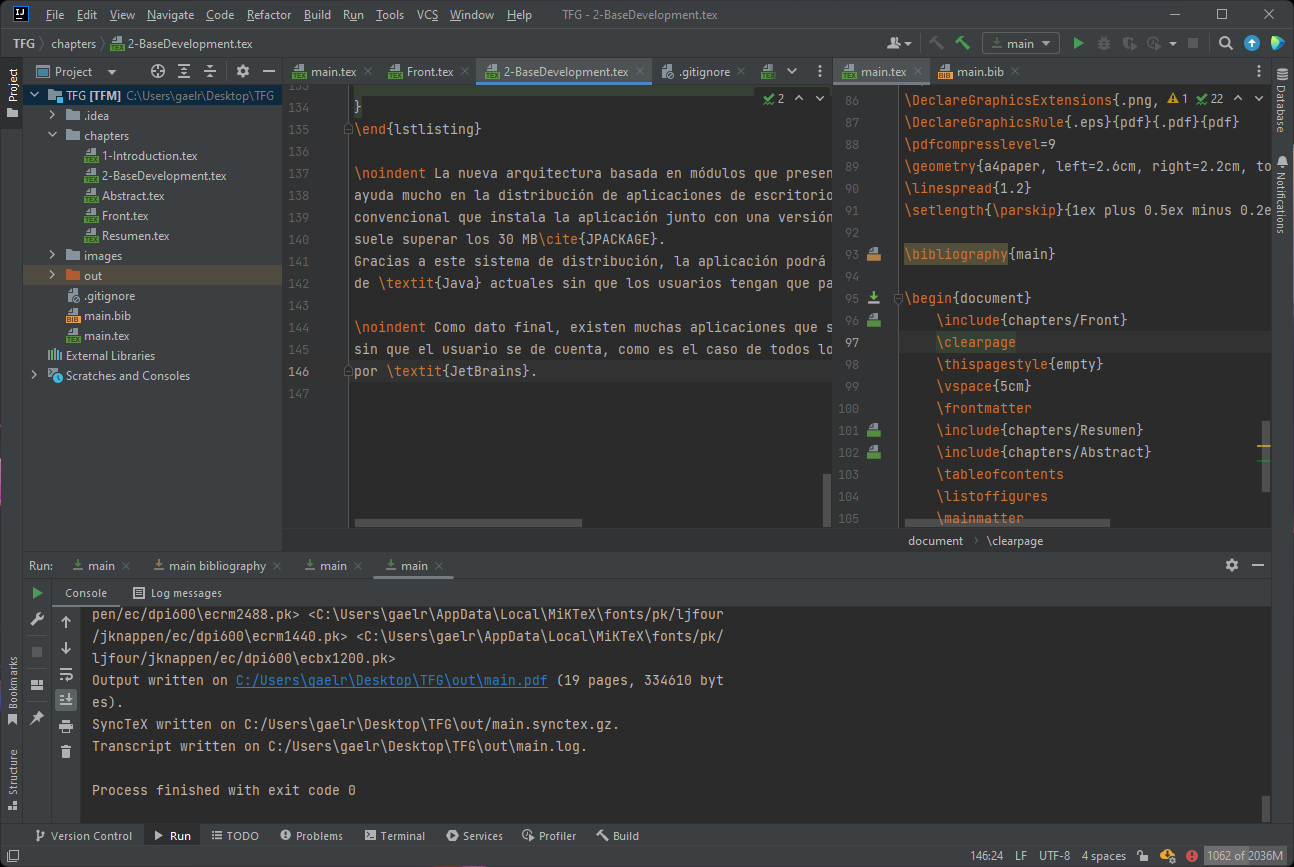
\includegraphics[width=\textwidth]{images/base/intellij-idea}
    \caption{\textit{IntelliJ IDEA}}
    \label{fig:java-intellij-idea}
\end{figure}


\section{Estructura del proyecto}\label{sec:estructura-del-proyecto}

\textit{JAMS} sigue los estándares de estructura de \textit{Gradle}\cite{GRADLE_ORGANIZING}.
Esto hace que su estructura sea muy similar a otras aplicaciones que usan el mismo
sistema de automatización.

\subsection{Tareas}\label{subsec:tareas}

El elemento más importante del directorio raíz es el archivo \textbf{build.gradle}.
En él se especifican las dependencias y se define cómo se debe compilar el proyecto.
Las \textbf{tareas} son las encargadas de definir dicho comportamiento.

Las dos tareas más importantes son las siguientes:
\begin{itemize}
    \item \textbf{jpackage:} permite generar un instalador de la aplicación específico
    para la máquina que ejecuta la tarea.
    \item \textbf{bundle:} genera un archivo \textit{jar} con la aplicación y todas
    sus dependencias.
    Este archivo puede ser ejecutado en cualquier sistema operativo que pueda correr
    \textit{Java} y esté soportado por \textit{JavaFX}.
\end{itemize}

Para ejecutar estas tareas ha de usarse el \textit{script} $gradlew$.
Este comando descargará \textit{Gradle} si es necesario y ejecutará
la tarea pasada como argumento.
Todos estos comportamientos están automatizados en \textit{GitHub}
mediante los \textit{scripts} dentro de la carpeta $.github$.

\subsection{Módulos y paquetes}\label{subsec:modulos-y-paquetes}

Dentro de la carpeta $src$ están definidos los dos módulos principales del
proyecto: $main$ y $test$.

El módulo $main$ es el encargado de almacenar todo el código fuente
de la aplicación.
Puede ser considerado el módulo más importante del proyecto.
El módulo $test$ define todas las pruebas unitarias que el módulo $main$
debe superar para que la aplicación se compile con éxito.

El código fuente almacenado en el módulo $main$ está separado en diferentes
paquetes \textit{Java}:
\begin{itemize}
    \item \textbf{collection:} contiene una serie de colecciones modificadas.
    \item \textbf{configuration:} contiene el sistema de configuraciones.
    \item \textbf{event:} contiene el sistema de eventos.
    \item \textbf{file:} contiene los tipos de archivo definidos en la aplicación.
    \item \textbf{gui:} contiene toda la interfaz de la aplicación.
    \item \textbf{language:} contiene el sistema de idiomas.
    \item \textbf{manager:} contiene el sistema de gestores.
    \item \textbf{mips:} contiene todas las herramientas relacionadas con la arquitectura \textit{MIPS32}.
    \item \textbf{plugin:} contiene el sistema de componentes.
    \item \textbf{project:} contiene el sistema de proyectos.
    \item \textbf{task:} contiene el sistema de hijos y tareas asíncronas.
    \item \textbf{utils:} contiene clases útiles utilizadas por los anteriores paquetes.
\end{itemize}


\section{Proyectos}\label{sec:interfaz-grafica}

\textit{JAMS} es un \textit{IDE} basado en \textbf{proyectos}.
Un proyecto está formado por una carpeta y una serie de propiedades
que son las siguientes:
\begin{itemize}
    \item \textbf{Tipo de proyecto:} especifica el tipo de proyecto.
    En una versión sin componentes este valor solo puede tomar el valor \textit{MIPS}.
    \item \textbf{Propiedades del proyecto:} parámetros necesarios por el tipo de proyecto.
    Configuran aspectos concretos y generales del proyecto en su conjunto.
    \item \textbf{Archivos para ensamblar:} lista de archivos que el ensamblador tendrá en cuenta
    al ensamblar el proyecto.
    \item \textbf{Configuraciones:} especifican propiedades \textbf{de la ejecución} del proyecto.
    Es decir, configuran el simulador.
    Un proyecto puede tener varias configuraciones, y el usuario ha de elegir una al crear una
    simulación.
\end{itemize}

Los proyectos son almacenados en carpetas.
Una carpeta de un proyecto tiene la siguiente estructura:

\begin{center}
    \basictree{
        [MyProject
        [.jams
        [data.json]
        [files\_to\_assemble.json]
        ]
        [Simulation Files
        [MySimulationFile.txt]
        ]
        [MyAsmFile.asm]
        ]
    }
\end{center}

Cada proyecto tiene dos carpetas por defecto: \textbf{.jams} y
\textbf{Simulation Files}.
La carpeta \textbf{.jams} contiene los datos del proyecto que \textit{JAMS}
gestiona de manera automática.
Esta carpeta está oculta y no debe ser modificada por el usuario.
El archivo \textbf{data.json} contiene el tipo de proyecto y sus propiedades,
mientras que \textit{files\_to\_assemble.json} contiene la listas de archivos fuente
que el ensamblador ha de procesar para crear la aplicación.
La carpeta \textit{Simulation Files} actúa de carpeta raíz del simulador:
todos los archivos que escriba o lea el simulador deben estar situados dentro
de esta carpeta.
